% !TEX TS-program = pdflatexmk

%----------------------------------------------------------------------------------------
%	PACKAGES AND OTHER DOCUMENT CONFIGURATIONS
%----------------------------------------------------------------------------------------

\documentclass[11pt]{diazessay} % Font size (can be 10pt, 11pt or 12pt)

\usepackage{listings}
\usepackage{color}
\usepackage{float}

\definecolor{dkgreen}{rgb}{0,0.6,0}
\definecolor{gray}{rgb}{0.5,0.5,0.5}
\definecolor{mauve}{rgb}{0.58,0,0.82}

\usepackage[sorting=none]{biblatex} %Imports biblatex package
\addbibresource{citations.bib} %Import the bibliography file
\usepackage{hyperref}
\usepackage{amsmath}

\usepackage{geometry}
\geometry{margin=1in}


%The special font for Java code
\lstset{frame=tb,
  language=Java,
  aboveskip=3mm,
  belowskip=3mm,
  showstringspaces=false,
  columns=flexible,
  basicstyle={\small\ttfamily},
  numbers=none,
  numberstyle=\tiny\color{gray},
  keywordstyle=\color{blue},
  commentstyle=\color{dkgreen},
  stringstyle=\color{mauve},
  breaklines=true,
  breakatwhitespace=true,
  tabsize=3
}
%----------------------------------------------------------------------------------------
%	TITLE SECTION
%----------------------------------------------------------------------------------------

\title{\textbf{Multi-label Image Classification with Deep CNN } } % Title and subtitle

\author{\textbf{Zijun Zhao, Dailun Li, Kaiwen Xu} } % Author and institution
%----------------------------------------------------------------------------------------

\begin{document}

\maketitle % Print the title section

%----------------------------------------------------------------------------------------
%	ABSTRACT AND KEYWORDS
%----------------------------------------------------------------------------------------

\begin{abstract}
In this project we investigate the performance of convolutional neural networks on the task of classifying multi-label image data. We develop a 12-layer CNN based on Alex-Net, which achieves around 94\% accuracy on the test dataset. After that, we further implement some creative strategies, including data augmentation, noise handling, drop out and usage of unlabelled data, to boost that score to above 96\%. Finally, we conclude and discuss where we can go beyond that score. \end{abstract}

%----------------------------------------------------------------------------------------
%	ESSAY BODY
%----------------------------------------------------------------------------------------

\section{Introduction}
Inspired by Alex Krizhevsky et al., whose groundbreaking research draw attention to deep convolutional neural networks \cite{Alex}, we want to utilize the powerful tool of deep CNN to solve some real world problems. The problem is to identify a combination of one handwritten digit and one handwritten english alphabet in a 56x56 image. We explore numerous convolutional neural network architectures and decide to develop a 12-layer CNN based on Alex-Net. Then we tune the hyper-parameters in our model so that both the validation accuracy and training speed are optimized.

\section{Datasets}
This dataset contains 30,000 samples, each sample is a 56x56 image. There're 30,000 labels accordingly. Each label is a size 36 binary vector. The first 10 binary values correspond to the digits 0-9, and the last 26 correspond to alphabet a-z. We use these data to train and validate our model. (Validation : Training = 0.01 : 1) We also have 30,000 unlabelled data, whose usage will be explored in the "Creative Work" section.
%------------------------------------------------
\section{Experimentation}

\subsection{Model Selection}
\begin{figure}[H]
	\centering
	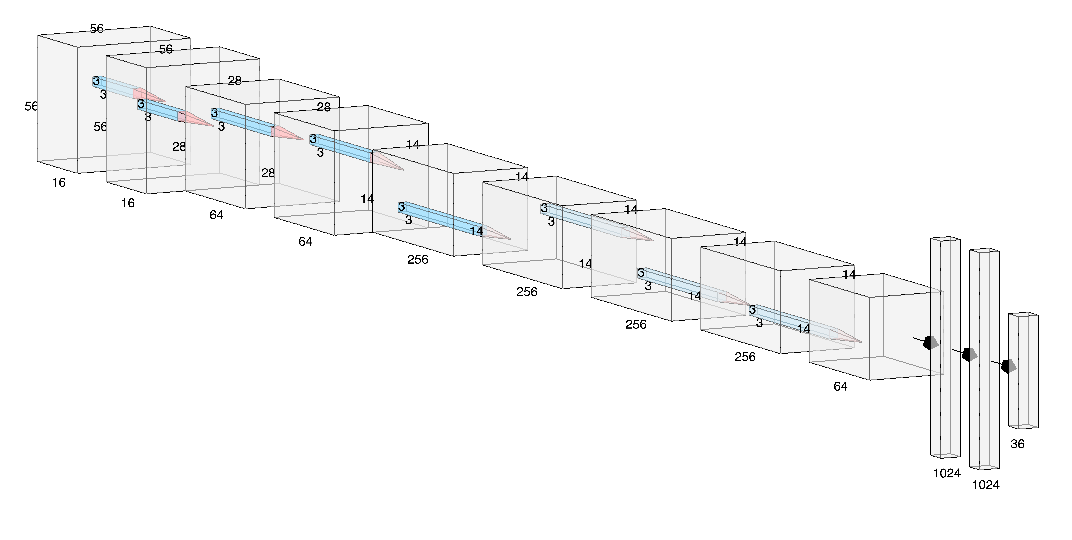
\includegraphics[width=0.7\linewidth]{net_structure.png}
	\caption{The architecture of our CNN}
\end{figure}

\subsection{Hyper-parameter tuning}

\begin{table}[H]
     \caption{Different Models with their parameters and performances}
        \label{preprocess}
    \begin{tabular}{ c c c c c c}
    \hline
    
     Model & $\#$ Conv layers & $\#$ Fc layers & Gradient Descent & Activation & Accuracy(train | test) \\
     \hline
    Naive Convnet  & 2 & 3 & SGD & ReLU & 0.85 | 0.08 \\
    Alexnet   & 4 & 3 & SGD & ReLU & 0.9 | 0.81\\
    VGG16  & 13 & 3& SGD & ReLU & 0.99 | 0.85\\
    DeepAlex & 9 & 3 & Adam & Leaky ReLU & 0.999 | 0.994\\
 
      \hline
    \end{tabular}
\end{table}

\subsection{Gradient descent parameters}
%------------------------------------------------
\section{Creative Work}
\subsection{Data Augmentation}
Although because of pooling layers, convolutional neural networks are inherently translation invariant, they are not invariant to rotational transforms (see appendix). As a result, we apply rotation of -30\textdegree, -15\textdegree, 15\textdegree and 30\textdegree to the training set to form a much larger dataset. We train our model on the new dataset. In this way, our model learns to identify labels with different rotations.

\subsection{Noise Handling}
We observe from the dataset that most of the images are noisy. Besides the digit and alphabet, we can also see intense unconnected dots, or slight speckle noise that covers almost the whole image. Initially, we try to remove these noise by applying filters before training, but we observe the validation accuracy to decrease. Inspired by Akbiyik's article on noise injection\cite{akbiyik}, we realize that random noises on training data actually help with the robustness of the CNN model we train. It regularizes the model, so that it does not overfit to the training data, and thus generalizes better. So we train with the original noisy data and filter out the noises only when we do prediction on validation and test data.

\subsection{Unlabelled Data}

%------------------------------------------------
\section{Conclusion and Go Beyond}


\section{Appendix}

\begin{figure}[H]
	\centering
	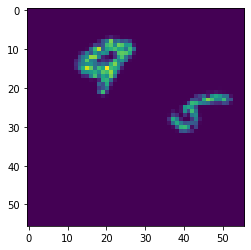
\includegraphics[width=0.5\linewidth]{5a.png}
	\caption{Skew digit and alphabet (5a)}
\end{figure}

\printbibliography %Prints bibliography


\end{document}
